\section[Collimators and Sieve Slits]{Collimators and Sieve Slits
\footnote{
  $CVS~revision~ $Id: slit.tex,v 1.7 2008/04/01 16:52:31 lerose Exp $ $ 
}
\footnote{Authors: J.LeRose \email{lerose@jlab.org}}
}

Both spectrometers have front-end devices for calibrating the optical
properties of the spectrometers. These are known as the collimator boxes.
These boxes are positioned between the scattering chamber and the 
first quadrupoles (Q1). Each box is carefully aligned and rigidly attached
to the  entrance flange of the Q1 of the respective spectrometer.  The boxes are
part of the vacuum system of the spectrometer.

Inside each box a ladder is mounted which is guided by a linear bearing
and moved up and down by a ball screw. On this ladder 3 positions are 
available to insert collimators. Below this ladder
a special valve is mounted that can isolate the vacuum in the spectrometer
from the target system. This valve should be activated when it is moved
in front of the holes connecting the box with spectrometer and target chamber.
\infolevone{
A schematic view of the collimator box is shown in Fig.~\ref{fig:coll}.

\begin{figure}
\begin{center}
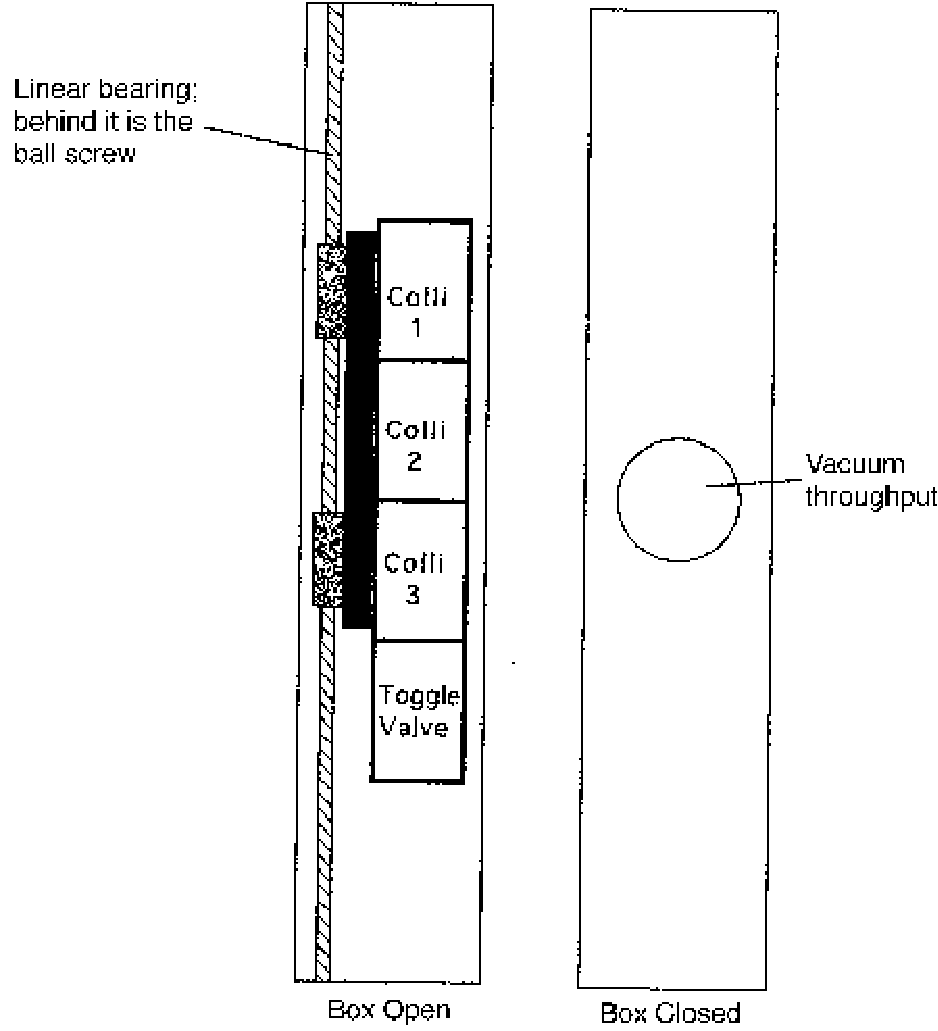
\includegraphics[angle=0,width=13cm,clip]{collimator_clip}
{\linespread{1.}
\caption[Spectrometers: Collimator Box Schematic]{Schematic layout of the collimator box.}
\label{fig:coll}}
\end{center}
\end{figure}
} %infolev

Vacuum requirement is $10^{-6}$ Torr. The material for the box is 
aluminum. It is possible to open one side of the box so that
collimators can be exchanged. The
reproducibility of collimator positions after moving
the ladder and/or after replacing a collimator is
better than 0.1 mm in horizontal and vertical direction.
The dimensions of the box are
roughly height=175 cm , width=35 cm and depth=15 cm.
The tolerance in the dimension
of the 7 msr collimator hole is $\pm0.5$ mm in each direction. 
The tolerance in the position
of each of the sieve-slit holes is $\pm0.1$ mm in each direction.

\infolevone{
\begin{figure}
\begin{center}
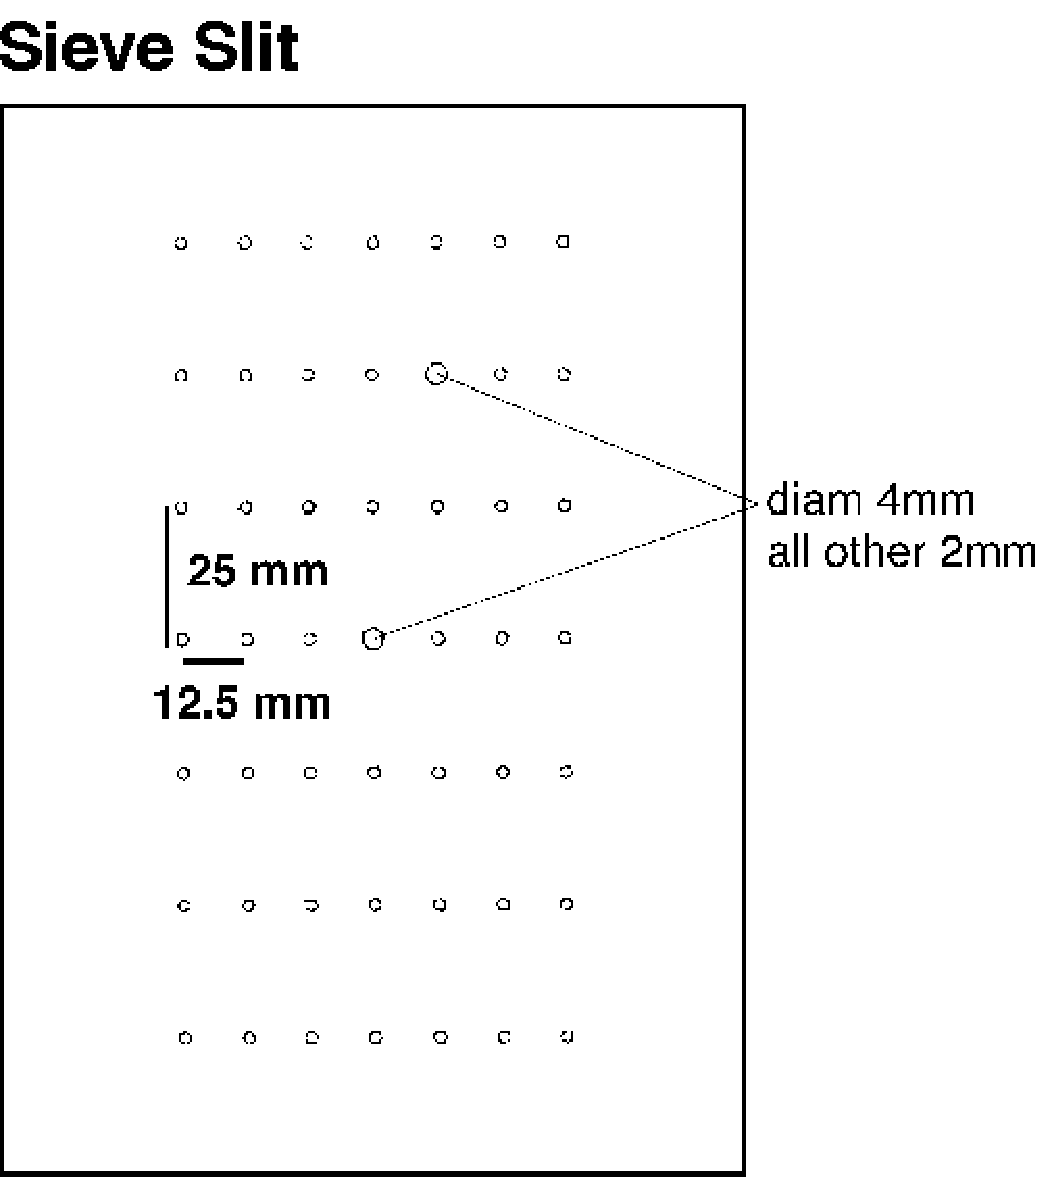
\includegraphics[angle=0,width=13cm,clip]{sieveslit}
{\linespread{1.}
\caption[Spectrometers: Sieve Slit]{Sieve slit collimator for optics calibration.}
\label{fig:sieve}}
\end{center}
\end{figure}
} %infolev
A typical sieve slit collimator 
\infolevone{(shown in Fig.~\ref{fig:sieve})
} %infolev 
consists of a plate of roughly 14 cm x 20 cm containing 49 holes
positioned in a regular 7x7 pattern. This slit is made out of 5
mm thick tungsten.
The holes have a diameter of 2 mm except for the central one and one positioned
off-diagonal which have a diameter of 4 mm. The horizontal distance between the
holes is 12.5 mm while the vertical distance is 25.0 mm.

To get the latest information on the dimensions and locations of the collimators see 
the Hall A homepage on the web%
\htmladdnormallinkfoot{}{\url{
http://hallaweb.jlab.org/
}}.

\begin{safetyen}{10}{15}
\subsection{Safety Assessment}

The collimator boxes form part of the vacuum system for each spectrometer. All hazards
identified in the spectrometer vacuum section apply to the collimator box as well.

In addition, safe access to the top of
the collimator boxes is needed  during manual operation of the box as outlined below.
Due to the proximity of the collimator boxes to the scattering chamber, and Q1 quadrupoles,
all necessary safety precautions with regards to vacuum windows, electrical power cables, 
cryogenic transfer lines, and high magnetic field should be taken. A radiological survey and
appropriate RADCON designated procedures must be followed when dealing with sieves 
and collimators.
\end{safetyen}

\infolevtwo{
\subsection{Operating Procedure}
Slit position is changed remotely from the standard Hall A control screen.
} %infolev

\begin{safetyen}{10}{15}
\subsection{Authorized  Personnel} 
\end{safetyen}
The authorized personnel is shown in table \ref{tab:slit:personnel}.
\begin{namestab}{tab:slit:personnel}{Collimator: authorized personnel}{%
      Collimator: authorized personnel.}
  \JessieButler{Mechanics and vacuum}
\end{namestab}

